\section{Resultados}
	
\subsection{Hardware}

	Como afirmado anteriormente, o primeiro passo do projeto é a prototipagem do Hardware do sistema, que inclui o Arduino, os botões e potenciômetros, através da plataforma online TinkerCAD, que inclui em si um monitor serial para visualizar o que está sendo enviado serialmente pelo microcontrolador.

\begin{figure}[htbp]
     \centerline{
        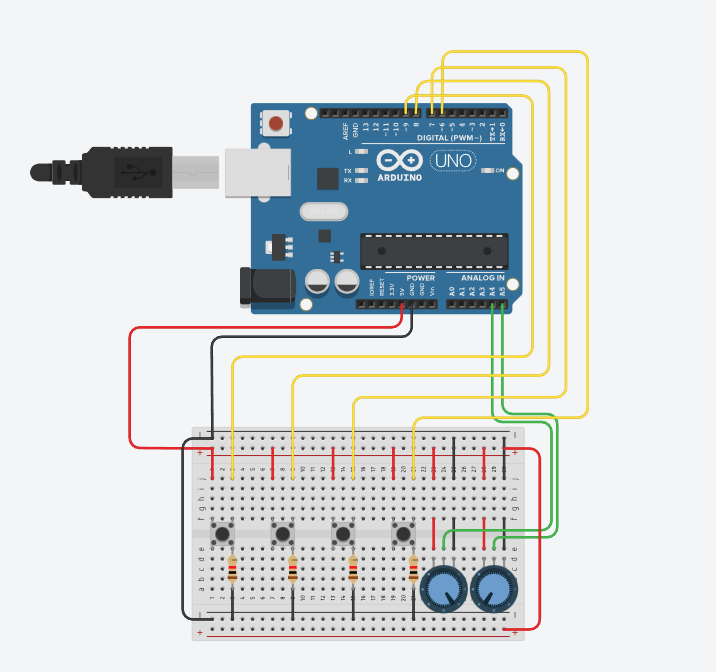
\includegraphics[width=2in]{tinkercad.png}
        }
     \caption{Modelo prototipado no TinkerCAD.}
     \label{fig}
    \end{figure}

	Como pode ser visto na figura acima, o modelo foi criado para abrigar dois potenciômetros e uma quantidade de botões, que foram 4 no momento da simulação. Cada um destes associados a um pino digital respectivo. Assim, a função do Arduino será pegar as informações desses componentes eletrônicos e enviar serialmente para o computador serialmente. O que tornará isso possível é a utilização da biblioteca "softwareserial.h" e suas funções, que possibilitam a comunicação.
	
	Para enviar todas as informações de uma única vez, em um pacote só, elas serão inseridas em uma string, e sua separação será realizada no código do Processing. Assim sendo, o código inserido no Arduino compreende a seguinte lógica:

\begin{lstlisting}[language=C]
const int pot1 = A5, pot2 = A3; //Potenciometros
const int b01 = 8, b02 = 7; // Botoes
int v_pot1 = 0, v_pot2 = 0; //Valores dos potenciometros
bool v_b01,v_b02; //Valores dos Botoes
int arr[10];

void setup() {
  Serial.begin(9600);
  pinMode(pot1, INPUT);
  pinMode(pot2, INPUT);
  for(int i = 7; i <= 8; i++){
      pinMode(i, INPUT_PULLUP);
    }
}

void loop() {
  v_pot1 = map(analogRead(pot1),0,1023,0,255);
  Serial.print(String(v_pot1) + "-");
  v_pot2 = map(analogRead(pot2),0,1023,0,255);
  Serial.print(String(v_pot2) + "-");
  v_b01 = !digitalRead(b01);
  v_b02 = !digitalRead(b02);
  Serial.print(String(v_b01) + "-");
  Serial.print(String(v_b02) + "\n");
  delay(50);
}
\end{lstlisting}

	Além da declaração de variáveis, alguns recursos foram utilizados para saber por exemplo, se um botão estava sendo pressionado. Como ele está pinado em uma porta digital, é possivel utilizar uma propriedade chamada "INPUT\_PULLUP"	para fazer essa distinção. Isso ocorre já que o botão está conectado a um resistor de "Pull-Up", que está inbutido no Arduino UNO, e quando vemos a expressão abaixo, significa que essa resistência irá impactar naquele input quando acionado, atuando como um inversor, para assim se obter um nível lógico alto quando o botão é pressionado:

\begin{lstlisting}[language=C]
pinMode(i, INPUT_PULLUP);
\end{lstlisting}

	Coletadas as informaçãos, elas são adicionadas a uma string de modelo: [x-x-x-x], e esta será separada por uma lógica criada na programação em Processing, transformando-as em chars, e associando-as às suas respectivas classes/variáveis.

	Por fim, para acomodar os potenciômetros e botões, foi impresso em 3D um modelo de controle "joystick" chamado "Paddle Game Controller" apropriado para o "Pong", visto abaixo:

\begin{figure}[htbp]
     \centerline{
        \includegraphics[width=2in]{botão.png}
        }
     \caption{Controle impresso 3D para o jogo.}
     \label{fig}
    \end{figure}

\begin{figure}[htbp]
     \centerline{
        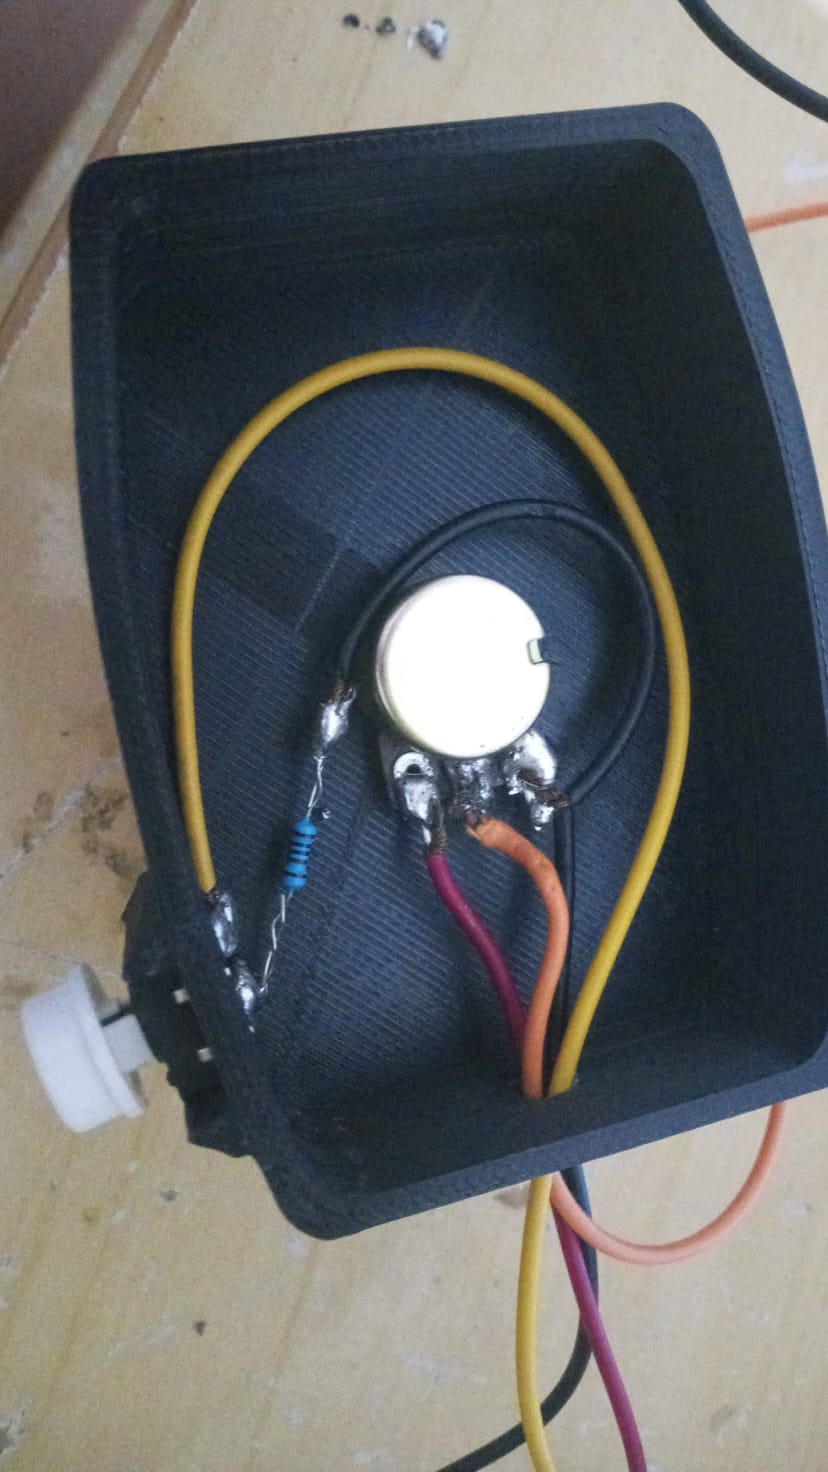
\includegraphics[width=2in]{solda.jpeg}
        }
     \caption{Eletrônicos soldados no controle.}
     \label{fig}
    \end{figure}

	

\subsection{Software/Processing}

	Antes de dar continuidade, é necessário estabelecer o que é desejado para o jogo: Uma tela inicial, que 
   pode levar ao jogo em si ou a um menu de instruções, e que o jogo possa ser pausado. Isso foi pensado ao longo do 
   desenvolvimento do jogo no qual, logo no inicio não tinha-se essa maturide, como pode-se observar na imagem abaixo:
	
	%%desenvolvimento

\begin{figure}[htbp]
     \centerline{
        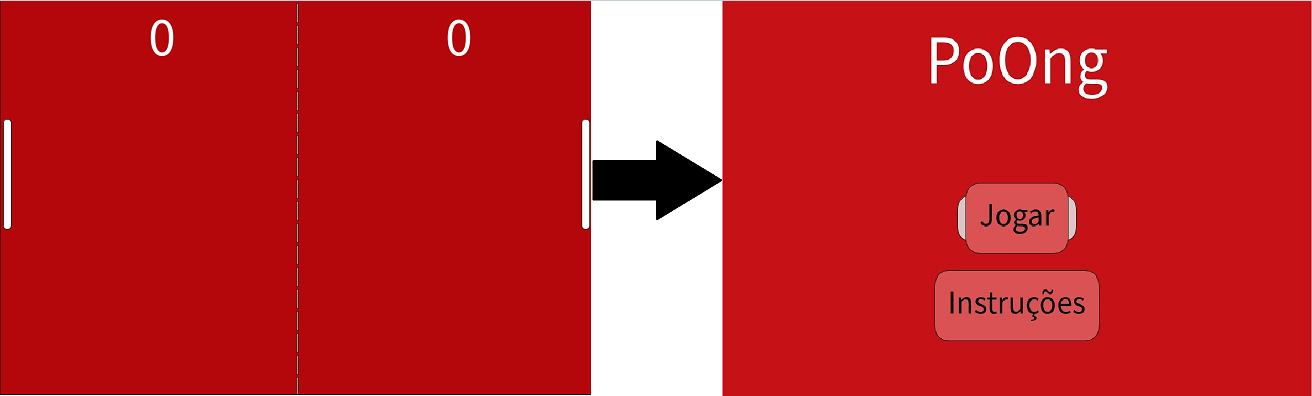
\includegraphics[width=5in]{evolucao.PNG}
        }
     \caption{Tela inicial do jogo.}
     \label{fig}
    \end{figure}
    
Essa tela inicial foi confecionada através do sofware processing, em que essa IDE posssibilitou o visualização e 
programação do jogo PONG. Portanto a lógica feita no programa foi a seguinte:

\begin{lstlisting}[language=C]
   void tela_inicial() { // Primeira tela
  pont1 = 0;
  pont2 = 0;

  background(200, 0, 0);
  textSize(height/6);
  fill(255);

  textSize(pulsando);
  text("PoOng", width/2, height/3 -150); // Textos finais
  if (pulsando == height/6 ) pulsando = height/7;
  else pulsando += 1;

  if (int(strBarra1) > 127 || int(strBarra2) > 127) jogar.select_bot();
  else instrucoes.select_bot();

  jogar.escreve("Jogar");
  instrucoes.escreve("Instruções");
\end{lstlisting}
Através dessa função é possivel definir a cor de fundo do game com o "background", a cor da letra com o "fill", 
como também qual local o texto irá ser alocado com o "textSize"  e especialmente determinar as opções da  tela principal,
que é "jogar"  e "intruções". Com isso, selecionando a tela de instrções é possível observar a seguinte imagem:

\begin{figure}[htbp]
   \centerline{
      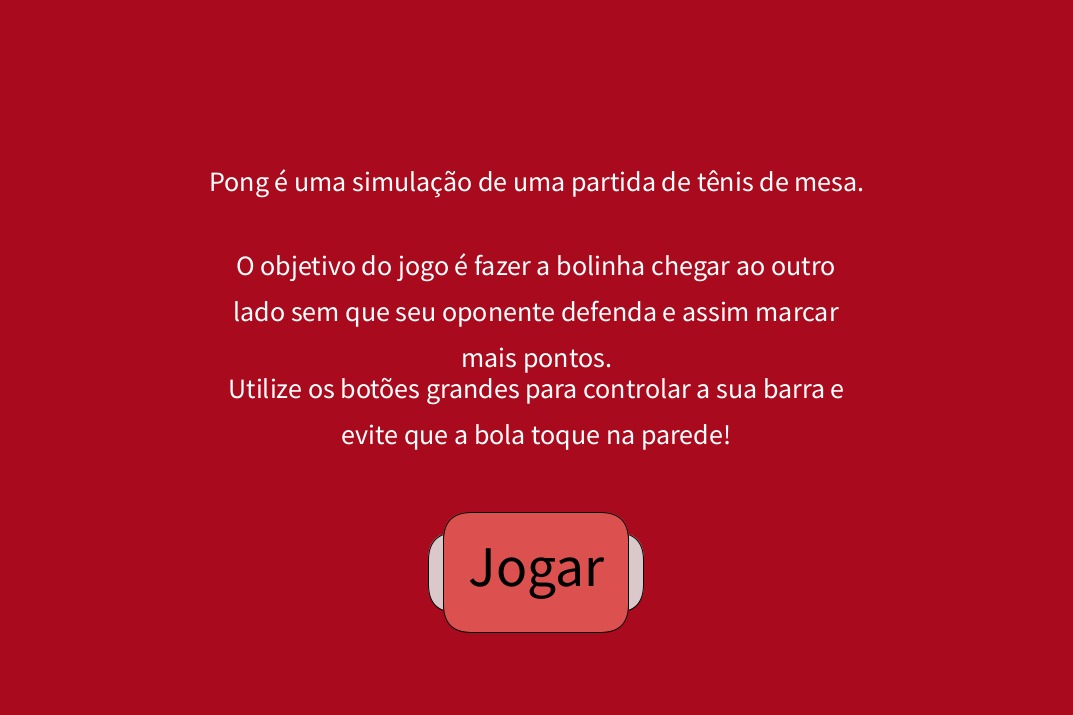
\includegraphics[width=4in]{instrucoes.jpeg}
      }
   \caption{Tela de instruções do jogo.}
   \label{fig}
  \end{figure}

Bem como sua programação, que é determinada por meio de uma estrutura textual do processing, como já citada anteriormente
denominada de"text"e caso a opção de "jogar" for selecionada o jogo inicia. Segue abaixo a lógica: 

\begin{lstlisting}[language=C]
   void tela_instrucoes() {
      background(170, 10, 30);
      textSize(height/25);
      fill(255);
    
      text("Pong é uma simulação de uma partida de tênis de mesa.", width/2, height/4);
    
      String s = "O objetivo do jogo é fazer a bolinha chegar ao outro lado sem que seu oponente defenda e assim marcar mais pontos.";
      text(s, width/2, height/2-50, width/2+100, height/2);
    
      String n = "Utilize os botões grandes para controlar a sua barra e evite que a bola toque na parede!";
      text(n, width/2, height/2+50, width/2+100, height/2);
    
      b3.select_bot();
      b3.escreve("Jogar");
    }
\end{lstlisting}

A tela de pause também teve sua evolução no decorrer do tempo, pois inicialmente não tinha-se tanta noção de como
fazer e configurar um game, mas no decorrer do desenvolvimento o conhecimento foi se aprimorando e como consequência
o jogo foi contnuando melhorando.

\begin{figure}[htbp]
   \centerline{
      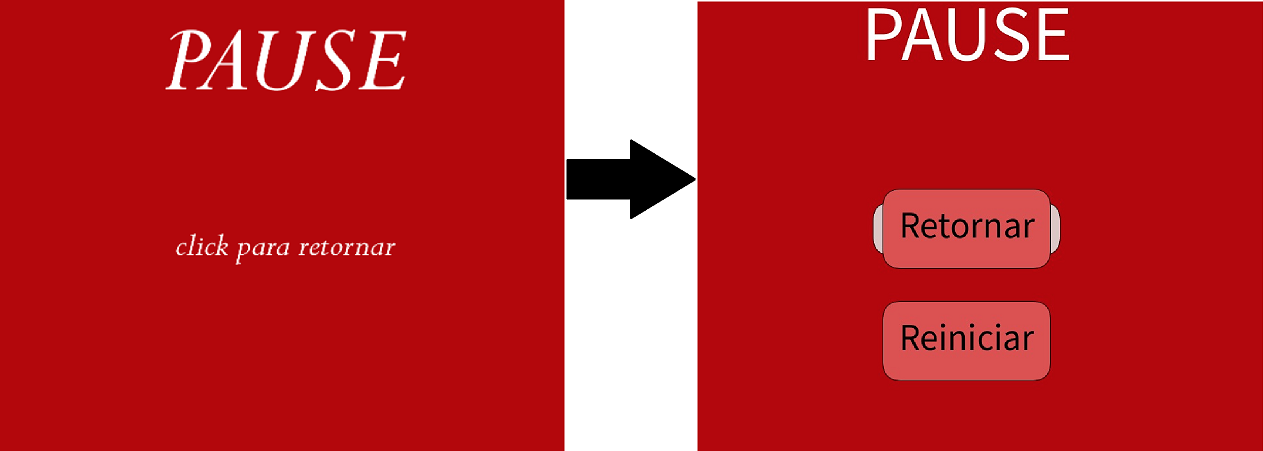
\includegraphics[width=5in]{tela-pause.PNG}
      }
   \caption{Tela de pause.}
   \label{fig}
  \end{figure}

  A tela de pause é acionada por intermédio de dois botões, na qual ambos jogadores tem que combinar a parada
  do jogo juntos e selecionar se querem retornar ao game ou reinicia-lo. Conforme o código abaixo:  

  \begin{lstlisting}[language=C]
   void tela_pause() { // Tela de pause do jogo

   background(180, 0, 0);
   textSize(height/6);
   fill(255);
   text("PAUSE", width/2, height/3 -200); // Textos de pause
 
   if (int(strBarra1) < 127 || int(strBarra2) < 127) retornar.select_bot();
   else reiniciar.select_bot();
   retornar.escreve("Retornar");
   reiniciar.escreve("Reiniciar");
   //text ();
 
   ordem = 3; //Mantém tela pause
 }
  \end{lstlisting}

  Como também a sua chamada no "draw", no qual é o loop onde o jogo roda.
  \begin{lstlisting}[language=C]
   case 3:
   tela_pause();
   if (click == 6 && (botao1.indexOf('1') != -1 || botao2.indexOf('1') != -1)) click = 7;

   if (click == 7 && (botao1.indexOf('1') == -1) && (botao2.indexOf('1') == -1)) {
     if (int(strBarra1) > 127 || int(strBarra2) > 127) {
       click = 4;
       ordem = 4;
     } else {
       click = 4;
       ordem = 2;
     }
   }
 }
  \end{lstlisting}

  Elaborou-se também uma tela  de vencedor, no qual exibe o vencedor da partida(esquerdo ou direito), essa função também sofreu alterações
  com o decorrer do tempo, conforme explicitado na imagem abaixo:
  
  \begin{figure}[htbp]
   \centerline{
      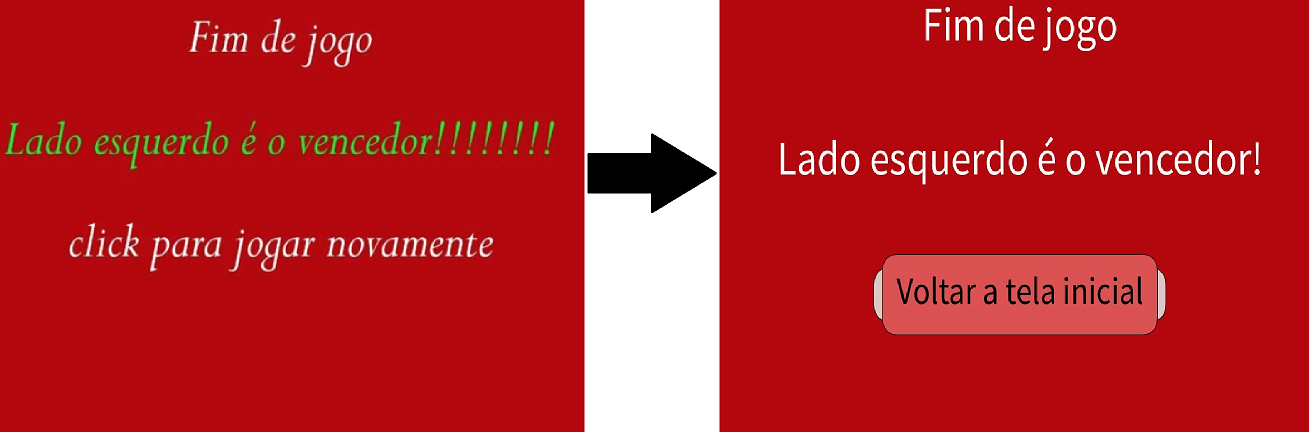
\includegraphics[width=5in]{tela-vencedor.PNG}
      }
   \caption{Tela de vencedor.}
   \label{fig}
  \end{figure}
Dessa forma foi definido um vencedor por intervenção da pontuação, ou seja, se o lado esquerdo estiver com uma maior pontução 
ele vence e acaba o jogo, de maneira analoga acontece com o lado direto se o mesmo obter mais pontos. Por fim o jogo
oferece a opção de retornar a tela inicial, de acordo com a lógica abaixo:
\begin{lstlisting}[language=C]
   void tela_pause() { // Tela de pause do jogo

   background(180, 0, 0);
   void fim_jogo() { // função de fim de jogo
   if (pontc2 == vencedor) { //definindo vencedor como um lado
     ganhou = "Lado esquerdo é o vencedor!";
   } else if (pontc1 == vencedor) { //definindo vencedor como um  outro lado
     ganhou = "Lado direito é o vencedor!";
   }
   background(180, 0, 0);
   textSize(height/10);
   fill(255); // definindo a cor das letras como brancas
   text("Fim de jogo", width/2, height/3 -200); // Textos finais
   text(ganhou, width/2, height/3);
 
   voltar.select_bot();
   voltar.escreve("Voltar a tela inicial");
 
   ordem = 4; // Mantem a tela final ativa
 }
  \end{lstlisting}

  Por último e mais importante, o jogo rodando, é importante salientar que o game em sua essência foi o mais modificado, não só 
  visualmente, mas principalmente logicamente, pois ocorreram diversas alterações até chegar a versão final, no qual não pode-se quantificar
  em imagens ou em números.


  \begin{figure}[htbp]
   \centerline{
      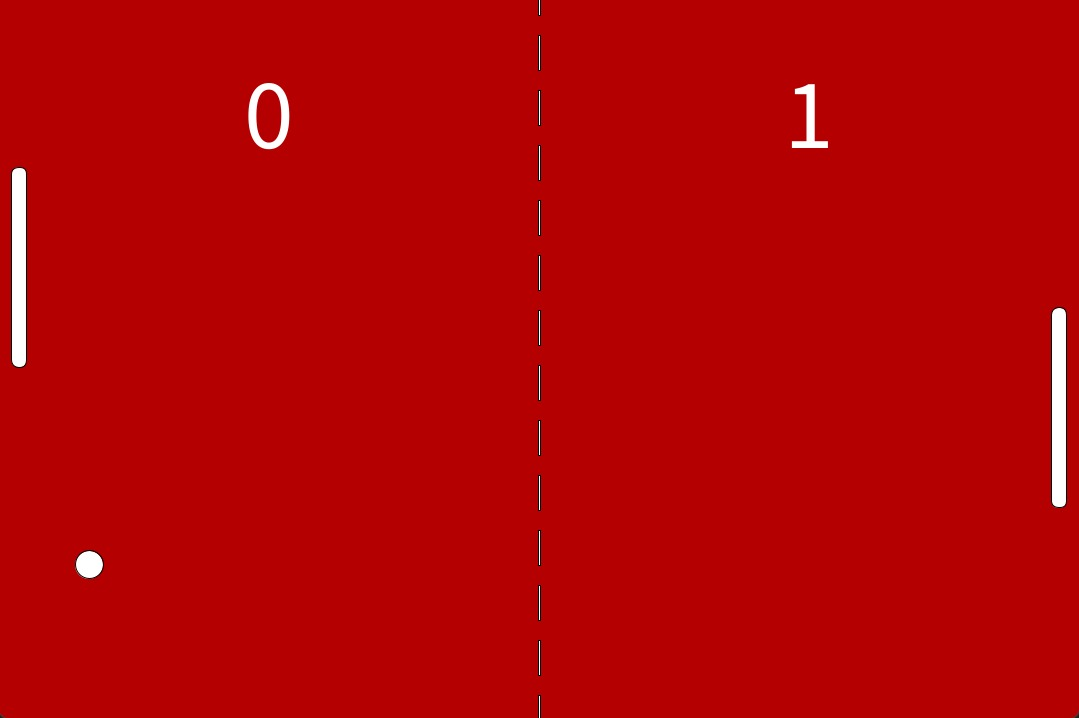
\includegraphics[width=3in]{jogo.jpeg}
      }
   \caption{Jogo rodando.}
   \label{fig}
    \end{figure}
\vspace{2cm}


    A dois obejtos principais para fazer o jogo PONG funcionar, que é as duas barras laterais e a bola, ambas tem
    uma física inerente para funcinar, bem como seus desenhos no game. Logo abaixo segue a codificação desses objetos
    que são utilizados como classes dentro do jogo:

classe da bola:
    \begin{lstlisting}[language=C]
      class bol { // Classe da bola

  float x, y; // Posicao da bola
  float xspeed = 5, yspeed = 2.3; //  Velocidade da bola
  float r = 14; //raio da bola

  bol() {
    x = width/2;
    y = height /2;
  }
  void display() { // Desenha a bola
    stroke(0);
    ellipse(x, y, 28, 28);
  }

  void move() { // Move a bola
    x += xspeed;
    y += yspeed;
  }

  void checkb() { // Checa se bateu em algum lugar
    if (x > width || x < 0) {
      xspeed = xspeed * (-1);
    }
    if (y > height || y < 0) {
      yspeed = yspeed * (-1);
    }
    
  }

  void checkpont() { // Aumenta a pontuação dos jogadores
    if (x == 0) {
      pont1 += 2;

      x = width/2;
      y = height/2;
      xspeed = xspeed * (-1);
    }
    if (x == width) {
      pont2 += 2;

      x = width/2;
      y = height/2;
      xspeed = xspeed * (-1);
    }
  }

  void colisaobarrad(float xx, float yy, float largura, float altura) {
    if (x + r > xx - largura/2 && y - r < yy + altura/2 && y + r> yy - altura/2) { // condições para a bola recochetear
      xspeed *= -1; // inverter a velocidade da bola
    }
  }

  void colisaobarrae(float xx, float yy, float largura, float altura) {
    if (y - r < yy + altura/2 && y + r > yy - altura/2 && x - r < xx + largura/2) { // condições para a bola recochetear
      xspeed *= -1; // inverter a velocidade da bola
    }
  }
}
    }
     \end{lstlisting}

 classe da barra:
 
 \begin{lstlisting}[language=C]
   class barra {

  float largura = 15;
  float altura = 200;
  float local_y = height/2; //posição y/2 para comerçar no centro da barra
  float local_x;

  barra(boolean esquerda) {
    if (esquerda) {
      local_x =  largura + 5; // o +5 serve para se afastar da borda
    } else {
      local_x = width - largura - 5;// o -5 serve para se afastar da borda
    }
  }

  void barra_inicio() { // configurando as barras iniciais
    fill(255);
    rect(local_x, local_y, largura, altura, 30);
  }

  void moverPot(int pos) {
    if (pos != local_y) {
      local_y = map(pos, 0, 255, 100, height - 100);  // Potenciometro
    }
  }
}
  \end{lstlisting}
